\chapter{智能，生于数学 \texorpdfstring{\\}{ }简明数学史}

\newenvironment{examplebox}
{\par\vspace{0.5em}\noindent\hrulefill\par\noindent{示例盒子：三跳链}\par\small}
{\par\noindent\hrulefill\vspace{0.5em}\normalsize\par}

%\begin{introduction}
%\item 萌芽：结绳计数与位值制
%\item 初等：几何、公理化与证明
%\item 近代：变量/函数、微积分与解析几何
%\item 现代：集合论、逻辑与可计算性
%\item 三次数学危机（无理数、微积分类基础、集合论悖论）
%\end{introduction}

% ChatGPT建议:保留纲要，微调条目措辞使并列更齐整，增加动词引导学习路径感。
% 修改后版本
\begin{introduction}
\item 萌芽：从结绳计数到位值制（建立“可表示与可计算”的底座）
\item 初等：几何、公理化与证明（从计算转向论证）
\item 近代：变量、函数、微积分与解析几何（刻画变化与空间）
\item 现代：集合论、逻辑与可计算性（统一基础与计算边界）
\item 三次数学危机：无理数、微积分基础、集合论悖论（以危机促重构）
\end{introduction}

\cnquote{"如果人们不相信数学很简单，那是因为他们没有意识到生活有多复杂。"}{ 约翰·冯·诺伊曼}

% ChatGPT建议:增加引导句，明确“读史的任务”与“线索三件套：表示—运算—证明”。
智能的历史可以追溯到人类最早期的思维活动，而数学是其中最重要的基础工具之一。为便于学习，我们按“萌芽—初等—近代—现代”的脉络，跟踪三条主线：\emph{如何表示}（符号与位值）、\emph{如何运算}（算法与优化）与\emph{如何确信}（证明与公理），看看它们如何在每一步为计算与智能埋下线索。

% ChatGPT建议:突出“需求→表示→规则化”的递进，并加一句引导“思考：为什么是位值而非重复”。
% 修改后版本
对于古代人来说，数字的诞生源于对数量的基本需求。  
从手指计数，到用石子、刻痕或结绳记录，人类在漫长的岁月中逐渐把具体的事物抽象为符号，再把符号提升为可计算的“数”。  
这种从经验到符号的演化并非一蹴而就，而是社会实践与思维试验长期积淀的结果。  
我们今天觉得“理所当然”的自然数，实则凝结着无数次的尝试与修正。  
正是这些早期的表征与规则，使“数量”第一次变得可表达、可运算，也让“可计算的表示”成为可能。

人类对"智能"的探讨源远流长。远在古希腊时期，哲学家们就已经开始追问：什么是智慧？什么是理性？我们如何通过思维去理解这个世界？从那时起，人们就梦想着创造能自主思考的机器：皮格马利翁（Pygmalion）、代达罗斯（Daedalus）、赫淮斯托斯（Hephaestus）等可被视为传说中的发明家，而加拉蒂亚（Galatea）、塔洛斯（Talos）与潘多拉（Pandora）则可被视为人造生命~{\cite{OvidMartin2004,Sparkes1996,Tandy1997}}。 \emph{这些想象后来在科学与工程中转化为“问题—表示—算法—数据”的框架，神话中的愿景开始落地为可检验的系统。}
% ChatGPT建议:保留神话例证，补一小句承上启下到“数学结构化”的方向。
%修改后版本
人类对“智能”的追问由来已久。古希腊哲学家求问智慧与理性的边界，神话中更不乏“人造生命”的想象：皮格马利翁、代达罗斯、赫淮斯托斯与加拉蒂亚、塔洛斯、潘多拉等~{\cite{OvidMartin2004,Sparkes1996,Tandy1997}}。这些想象在近代被抽取为\emph{问题—表示—算法—数据}的工程框架，逐步落地为可检验的系统，也把讨论引向一个关键：\emph{以数学进行结构化表达}。

这些问题不仅关乎哲学，还对现代科学和技术的发展产生了深远影响。随着时间推移，这种对智能的追问从哲学的纯理论思辨，逐渐转向了科学与工程的实践领域。早期的数学家如欧几里得、阿基米德以及笛卡尔等，通过逻辑和结构化的思维方式，为计算与智能提供了基础：欧氏公理化对应模型的可验证性；笛卡尔坐标促成连续空间的特征化；阿基米德近似展示了可计算思想的雏形。数学逐渐从实用算术走向系统推理，成为连接抽象理念与工程实现的桥梁。

% ChatGPT建议:并列点更工整；用“从……到……”加强演进节奏；句末回扣“桥梁”并加思考句。
% 修改后版本
这些问题不仅属于哲学，也深刻影响了现代科学与工程。追问的重心逐步从思辨转向实践：欧几里得以公理化对应\emph{可验证的模型}，笛卡尔以坐标系刻画\emph{连续的空间}，阿基米德的极限思想展现\emph{可计算的近似}。数学由此从实用算术走向系统推理，成为贯通抽象理念与工程实现的\emph{方法之桥}。（思考：当“可验证”“可表达”“可计算”三者冲突时，我们如何取舍？）

数学的发展史可以粗分为四期：萌芽、初等、近代与现代。这些分期并非泾渭分明，而是层层叠加与概念外延的扩展。\emph{为把握演化主线，接下来我们依次回顾四个阶段的关键观念与方法，并在节末用 \texttt{examplebox} 收束为“AI 建模要点”。}

% ChatGPT建议:保留结构声明，加入“学习导航”语气，提示读者关注“关键概念→AI映射”。
% 修改后版本
数学的发展可粗分为四期：萌芽、初等、近代与现代。分期并非泾渭分明，而是层层叠加、外延拓展。为把握主线，接下来我们按阶段提炼\emph{关键观念与方法}，并在每节以 \texttt{examplebox} 收束为“AI 建模要点”，帮助你把历史概念映射到当代智能的要素上。


\section{萌芽时期：从计数到位值制}

数学的萌芽时期从远古时代延续至公元前5世纪，是人类最早利用数学工具应对日常生活需求的阶段。通过手指计数、刻痕和结绳，人类逐渐形成自然数的概念与四则运算雏形，为后续的几何与代数提供了素材和直觉。\emph{总体上，这一时期以“就事论理”的经验法则为主，但已显露出从数与形中提炼稳定规则的趋势。}


 % ChatGPT建议:在段首点明“本节目标=从需求到表示”，在段尾加一句回扣“AI中的表示与编码”。
% 修改后版本
本节聚焦一个朴素但关键的问题：\emph{人类如何把“需求”变成“可表示、可计算的数量”？} 从远古至公元前5世纪，手指计数、刻痕与结绳支持了自然数与四则雏形的形成，为几何与代数提供了直觉与素材。总体看，这仍是“就事论理”的经验阶段，但已有从“数”与“形”中提炼稳定规则的趋势——这正是后世\emph{表示与编码}思想的源头。

\subsection{史前数学：日常需求与实用计算}


在公元前5世纪之前，数学并非独立学科，而是伴随人类生活的需求逐步发展的：牲畜计数、土地丈量、历法制定与贸易核算等场景催生了各种方法。古代美索不达米亚与埃及的泥板和石刻清楚记录了这些活动，展现了数学与生活实践的紧密联系。

% ChatGPT建议:用“场景串联→证据”结构；末句加“抽象线索”引导下一段实例。
% 修改后版本
在公元前5世纪之前，数学并非独立学科，而是服务于具体场景：牲畜计数、土地丈量、历法制定、贸易核算等。美索不达米亚与埃及的泥板、石刻为此提供了直接证据，展示了\emph{实践—记载—规则}的形成路径。由此抽离出的“\emph{稳定表示与可复用方法}”，成为迈向抽象的第一步。

“数学”活动最古老的痕迹之一是在美索不达米亚发现的一块泥板（约公元前2500年）。泥板记录了这样一个计算：如果谷仓里有 1\,152\,000 份粮食，每个人分得 7 份，一共可以分给多少人？结果是 164\,571 人，即用 1\,152\,000 除以 7 的结果。这说明在算术“成书”之前，美索不达米亚的会计师们已经能熟练地进行除法运算。甚至，书写完全有可能就是为了记账才发明的---若真如此，数字就比字母发明得还要早了。

② % ChatGPT建议:精炼数字叙述的节奏，突出“运算已先于理论成书”的结论。
③ 修改后版本
一个典型例证来自约公元前2500年的美索不达米亚泥板：记录了将 1,152,000 份粮食按每人 7 份分配的除法计算，答案为 164,571。这个细节表明，在算术“成书”之前，会计实践已相当成熟；甚至书写本身可能因记账而生——若如此，\emph{数字的历史或早于文字}。

古埃及人发展了基础的几何公式，在建造金字塔时已经能够运用高度和角度的几何关系；美索不达米亚的会计师不仅掌握了加法和乘法，还能解简单的二次方程，用于管理粮食和资源。巴比伦人对天体运动的观察与历法推算也推动了数学的发展。为了精确预测日食、月相以及制定历法，天文学家需要处理大量的时间和角度计算。这些天文观测不仅进一步提升了对测量和计算的要求，也推动了几何与代数的发展。

② % ChatGPT建议:并列更对称，句尾落到“从经验到模型”的抽象点，为后续“位值制”铺垫。
③ 修改后版本
古埃及在金字塔工程中发展了高度与角度的几何关系；两河流域的会计实践不仅熟练四则，还能求解简单二次方程以管理物资；巴比伦的天文历法为预测日食、月相而系统处理时间与角度。由此，\emph{测量—计算—规则}逐步汇聚为\emph{从经验到模型}的过渡，为更高效的\emph{表示系统}（位值制）铺垫了需求。

总体而言，这一阶段的数学活动是解决问题的经验性工具，尚未形成系统理论，但奠定了“数”与“形”的概念基础。这些先于理论的操作共同催化出对“可复用规则”的渴望，从而引向更稳健的记数手段。问题也由一次性的分配与测度，转向对“如何表示与传递数量”的一般方法。

② % ChatGPT建议:段尾加入“学习回顾句”，回扣导览中“表示与运算”的目标。
③ 修改后版本
总体来看，这一阶段仍以经验工具为主，虽未成系统理论，却稳固了“数”与“形”的概念根基。先于理论的操作催生了对“可复用规则”的渴望，问题由一次性分配与测度，转向\emph{如何表示与传递数量}的一般方法。小结：请把握“\emph{需求→表示→规则化}”这条线索，它将在后续位值制与算法化中反复出现。

%下节转向最朴素也最普及的载体---手指计数。

\subsection{手指：长在身上的计数器}

相信你在许多影视剧中都见过这样的一幕：一位算命先生，掐指一算，口中念念有词。这种“掐指一算”看似神秘，实则源自于古老而简便的计数方法。
\begin{figure}[htbp]
\centering
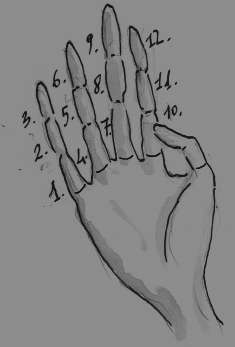
\includegraphics[width=0.3\textwidth]{figs/fingers.png}
\caption{“掐指一算”}
%\label{}
\end{figure}
在远古时代，用手指计数是再自然不过的选择，手指是人类最早的“随身计算器”。它帮助人们轻松应对日常计数需求，如记录牲畜数量、物品交换量，推算季节与节气，安排农耕节日等活动。由此，一个从身体到符号的过渡被打开：手指结构为进制与位权提供了直觉。

手指的构造与多种进制系统有着天然的联系。稍加思考，我们就能找到十进制、二十进制、十二进制等计数法与手指构造的对应关系。
十进制(Decimal System)是最常见、最自然的计数方式，与双手十指自然对应。十进制系统在全球的广泛使用，源于人类天生拥有十根手指的解剖学特征。正如爱德华·卢卡斯所言，这是“自然界的一个偶然事件”​。
十二进制(Duodecimal System)则适用于更复杂的计数需求。除大拇指外，四根手指各有三段指节。一只手的大拇指轮流指向其余四根手指的各段指节，可以计数1到12。这种方式在古代美索不达米亚和古埃及广泛应用，至今仍用于时间和角度的计数系统中，如12小时制、一年12个月等。
六十进制(Sexagesimal System)则更加复杂。它结合双手来计数。一只手用于计12（与十二进制相同），另一只手的五根手指则记录12的倍数，五轮12等于60。六十进制在古巴比伦时期被发明，沿用至今，广泛用于时间和角度的计量，例如1小时=60分钟，1分钟=60秒，以及360度的圆周划分。
二十进制(Vigesimal System)也是一种古老的计数法。为了更大范围的计算，一些古代民族不仅用手指，还加上脚趾来计数。例如，中美洲的玛雅文明和阿兹特克文明，以及现今的西非和欧洲部分地区，采用了以20为基数的计数法。
二十进制的痕迹在许多语言中依然存在。现代英语中的"score"表示20的用法便保留了这一印记。
例如，莎士比亚在《圣经》英译本中使用“three score and ten”（20的3倍加10，表示70岁)来指代古稀之年；林肯在《葛底斯堡演讲》中使用“four score and seven years ago”(20的4倍加7，表示87)来表达87年前的历史。一百年后，马丁·路德·金在其著名的演讲《I have a dream》中说“Five score years ago”​（20的5倍，即100年前）​。
英国曾有一个\emph{12 与 20 进制组合}的货币系统：1英镑=20先令，1先令=12便士。1971年，英国引入了十进制货币系统，1英镑=100便士，先令在1990年后彻底退出流通。
在法语、丹麦语和巴斯克语中也能找到二十进制的痕迹。例如，法语中的数词从quatre-vingts(80)​、quatre-vingts-dix(90)​，到quatre-vingts-dix-neuf(99)。同时，这些语言中还混杂了六十进制的痕迹，如数词soixante(60)到soixante-dix-neuf(79)。
手指不仅是身体的一部分，还是人类最早的天然计算工具。它帮助我们理解和组织世界，并为现代数学中的位值制和进制系统提供了最初的灵感。直到今天，手指仍是许多人在进行简单计算时的本能工具。


\subsection{荒岛上的自然教育，人类数字文明的缩影}
设想你在一次航海探险中遭遇风暴，不幸漂流到了一个无人岛。没有手表和手机，也没有任何现代工具。你很快面临一个问题---如何计算时间？如何记录每天收集的食物？在这种完全回归自然的环境中，你必须依靠最原始的方式来解决这些问题。这个经历，其实正是早期人类如何发明和发展数字的缩影。

\subsection{手指计数：最简单的工具}

为便于阅读，本节（手指计数：最简单的工具）承接上节（荒岛上的自然教育，人类数字文明的缩影），先交代差异与共同点，再聚焦本节关键问题。

你的第一反应可能是用手指来计数。十根手指天生就是人类最便捷的“计算器”，帮助你快速记录简单的数量---比如你捕到的鱼或采摘的果实。手指计数是直观而方便，几乎无需思考就能完成。但很快，你意识到这种方法有明显的局限性：当数字变大，或需要记录更复杂的信息时，手指显然不够用了。更重要的是，手指计数无法保存这些数据，一旦忘记，你的记录便随之消失。{（抽象：易得的“工作记忆” vs. 可复查的“外部记忆”。）}

\subsection{刻痕计数：更长久的记录方式}

为便于阅读，本节（刻痕计数：更长久的记录方式）承接上节（手指计数：最简单的工具），先交代差异与共同点，再聚焦本节关键问题。

为了更长久地保存记录，你开始在岛上的树木或石头上刻下痕迹。每道刻痕代表一天的过去，或你每天捕获的鱼或采摘的果实数量......。刻痕计数法让你能够更长久地保存这些信息。每天的刻痕不断累积，形成一个记录时间和活动的系统。这种方法虽然简单，却比手指计数更加持久、可靠，也能应对稍微复杂的需求，比如记录日期或特定的事件。然而，随着时间的推移，刻痕的数量增加，管理这些信息变得越来越困难。你开始需要一种更便捷、更灵活的方式来记录和传递这些信息。{（AI 启发：从短上下文到外部存储/检索---RAG 的原型。）}

\subsection{结绳记数：更高级的记数法}

为便于阅读，本节（结绳记数：更高级的记数法）承接上节（刻痕计数：更长久的记录方式），先交代差异与共同点，再聚焦本节关键问题。

幸运的是，你发现了一根绳子，这给了你一个新的选择---结绳记数法。通过在绳子上打不同的结，你可以标记不同的天数、事件或物品的数量。不同形状和位置的结可以表示不同的信息。相比于刻痕，结绳计数法更便捷灵活，更易于携带和传递，成为你在荒岛生活中的高级计数工具。{（抽象：符号化与压缩编码；启发：离散化/量化。）}

你在荒岛上的探索，正是人类数字文明进化的缩影。无论是刻痕还是结绳，这些方法都体现了人类从最初的物理标记到复杂符号系统的演化路径。通过这些自然的计数方法，你逐步掌握了记录、比较和计算的基本概念。这不仅是你个人的“自然教育”，也是数字发明的最初动力---让生活更加便捷和高效。{（一句话抽象：需求—表示—外部化—标准化的演化链。）}
从需求出发，人的记数方式沿着“即时—留痕—编码”的路径外化与标准化。下文据此上升到一般而稳定的表示---位值制。

\subsection{数字的位值系统}

在人类早期文明中，简单的手指计数和结绳、刻痕等方法已广泛用于记录数字。然而，随着社会发展，这些物理标记在处理更复杂和更大范围的数字时，显得低效而繁琐。于是，更加抽象的符号系统应运而生，催生了{\bf 位值制}这一革命性的数字表示方式，使得复杂的数值能够通过简单的符号位置来表示和计算。
早期的计数系统大多采用{\bf 加法规则}。例如，在古代巴比伦的黏土板上，数字是通过符号的重复来表示的：数字“1”用一个符号表示，数字“2”用两个相同符号表示，数字“3”则用三个相同符号。
这种计数方式在中文数字、罗马数字、古印度的婆罗门数字和笈多王朝使用的数字，以及大洋彼岸的玛雅数字中都很常见。大多数古代文明在表示前三个数字时，都采取了同样的方式：重复表示“1”的符号一次、两次、三次。古代的中文“一、二、三”、钟表盘上的罗马数字“~Ⅰ、Ⅱ、Ⅲ”、阿拉伯数字也体现了同样的重复方式。可是，从数字4开始，所有的文明就都放弃了这种重复。为什么呢？
研究发现，人类的数感对少于3的数字有天然的反应，但超出这个范围后，单纯的重复符号便变得困难。对一些出生几个月的婴孩进行试验，结果证实人类与生俱来的数感的容量不超过三。
试想一下，数字13若用重复排列“1”的符号13次来表示，无论是对书写还是阅读，都会很低效---怎么能一眼就看出它是13，而不是12或者14呢？
类似的问题在罗马数字系统中也很常见。罗马数字系统中，V表示5，X表示10，L表示50，C表示100。此外，向右添加符号为加，如，VI表示数字6，XI表示数字11；相反地，向左添加一个更小数值的符号为减，如IV表示4，IX表示9。
尽管使用了加减法规则的计数系统十分直观，但在表示大数时显得十分低效。例如1888年写成罗马数字就是MDCCCLXXXVIII，甚至无法有效表示类似100万那样的数字---除非把1000个M排成一排！

早期加法型记数（如罗马数字）在表达大数与运算效率上受限。位值制用“位置决定权重”的方式，以极少符号表达极大数量，长度近似 $\log x$。这不仅简化书写与计算，也带来压缩与编码的思想（最短码长度 $\approx-\log p$）。\emph{位值制因此成为现代信息处理与计算架构的共通底座。}
随着人类文明的发展，许多地区开始引入更为先进的计数法，其中最具革命性的是{\bf 位值制计数法}。古巴比伦、中国，尤其是印度和阿拉伯，率先采用了这种创新的位值制计数法。
这种计数法的关键在于符号的位置决定了其数值。例如，数字“12”和“21”虽然使用相同的符号，但因为符号位置不同，代表的数值也不同。
位值计数法具有出众的简洁性。
通过有限的符号，可以表达任意大的数值。
例如，$10^{100}$这个超出了物理限制的天文数字，在位值制下仅需101个符号即可表示---一个"1"后面跟着100个"0"。位值计数法用极短的符号链表示极其巨大的数值。
位值制不仅提高了数字的表示效率，还反映了数字的{\bf 对数增长}特性，即随着数字的增大，所需的符号长度呈对数增长，符号数量远远少于数字本身的大小。例如，表达$10^{100}$所需的符号长度约为$\log_{10}(10^{100})=100$。
一般地，表达任意整数 $x$所需的符号数量接近${\log_{10} x}$。

因此，从某种意义上，位值计数系统是最简洁、甚至最优的。{（信息论视角：最短码长度 $\approx -\log p$。）}
位值制的引入是人类计数方法的一次重大飞跃。从简单的重复符号到高度抽象的符号系统，位值制极大简化了计算过程，推动了计算和数学的发展，奠定了现代数字系统的基础。{（一句话抽象：位权 $\Rightarrow$ 表达与计算的指数增益；AI 启发：词表/位宽/量化。）}

\subsection{位值制与对数增长在现代计算机中的应用}

在计算机科学中，在已经排好序的数组中查找某个元素的时间也是数组长度的对数。即使数组规模如同宇宙般庞大，经过几百次迭代后，便能够找到所需的元素---唯一的限制就是光速有限性所带来的信息传播和处理速度的物理极限。
互联网的URL是位值制与对数增长在数据处理和网络寻址中的一个典型应用。一个简短的URL(Uniform Resource Locator，URL，统一资源定位符)迅速定位到海量信息。
想象一下，你希望在网上搜索某项信息。尽管互联网上的数据量可能以EB($10^{18}$字节)甚至ZB($10^{21}$字节)计量，只要拥有对应信息的URL，你几乎瞬间就能找到目标信息。
这正是对数增长的强大之处：即使面对巨大规模的数据集，只需少量步骤就能完成检索。
此外，URL的简短程度令人惊叹，其长度是整个网络大小的对数！这意味着我们可以轻松将URL存储在内存中，而URL指向的信息量却远远超出了其自身长度。
这种简洁有效的特性，展示了对数增长在计算与信息处理中的关键作用。
IPv4和IPv6的设计正是对数增长在实际应用中的另一个实例。
 IPv4地址使用{\bf 32位}二进制数来表示，每个IP地址可以被写成4个以点分隔的十进制数（如192.168.1.1），每部分对应一个8位的二进制数。

32位的二进制能够生成$2^{32}$，即约{\bf 43亿}个唯一IP地址。这在IPv4设计之初被认为是足够庞大的数目。然而，随着互联网的迅速扩展，特别是物联网（IoT）设备和移动设备的广泛普及后，IPv4的43亿个地址空间将很快耗尽。
   为了解决这一问题，{\bf IPv6}应运而生。IPv6使用{\bf 128位}二进制数表示，由八组以冒号分隔的16进制数构成(如 2001:0db8:85a3:0000:0000:8a2e:0370:7334)。这种128位的二进制表示能生成$2^{128}$，即约{\bf $3.4 \times 10^{38} $} 个唯一IP地址，相当于为地球上的每粒沙子分配多个IP地址。这一数量级足以应对未来几十年甚至几百年内所有联网设备的需求。
IPv4和IPv6的位数与它们能够支持的地址数量之间的巨大落差，展示了对数增长的强大力量。IPv4仅用32位符号就能表示43亿个地址，而IPv6仅用128位符号就能支持{\bf $3.4 \times 10^{38}$}个地址。随着位数的增加，IP地址系统实现了指数级的扩展，同时保持了地址表示的简洁性。{（AI 去向：索引结构/向量检索/稀疏路由—见 8.2、8.5。）}
% （去重）删除原文末尾对“二分查找/URL/IP”的再次并列复述，避免与上文重复。
%\emph{下一节我们从“表示的效率”转向“表示的抽象度”。}

\subsection{数字：从具象到抽象}

几千年来，人类都在探索如何建立数与物的对应关系，现代数字系统的定义正是基于这种探索的延续。一旦人类掌握了计数，数字系统的应用就变得“自然而然”了。或许正因如此，我们才称自然数为“自然”数(natural number)。然而，实际上，数字的概念一点也不“自然”。
无论是在早期人类在骨头及木棍上有序地刻下划痕，还是结绳或是在容器中放置物品无论是结绳，这些早期方法已代表了相当抽象的符号系统，其中抽象的数学对象与自然中的实际物体之间的分离，同一个数字既可以表示动物的数量，也可以记录借贷量或一个月的天数。
自此之后，数学研究的对象不再是必须与实际物体相关的几何图形和数字。研究对象性质的变化，最终引发了解决数学问题的方法的革命。{（AI 启发：可迁移表征与多任务共享—抽象层提高，泛化/可解释间的取舍加剧。）}
抽象提高了可迁移性，也带来语义漂移与解释性的张力。


\section{初等数学时期：从计算到推理}

公元前5世纪开始，数学进入了初等数学时期。这个时期的数学探索更加系统和深入，尤其是在欧几里得几何和代数方程的研究中，数与形的关系得到了更加严谨的探讨，算术、几何、代数和三角等数学分支逐渐成形。
公元前5世纪起，欧几里得几何与代数方程的研究使数与形的关系走向严密，算术、几何、代数与三角逐渐定型。核心转变在于：从求值走向论证，从技巧走向体系。
数学作为一种学科，经历了漫长的演化过程。起初，数学的诞生是为了解决生活中的实际问题---如何计数、测量、交易、管理时间等。在公元前5世纪之前，埃及和美索不达米亚等古老文明的数学发展更多地依赖于经验和实际操作，主要集中于如何进行计算，服务于土地测量、建筑工程、会计管理以及天文学等日常需求.
% （去重）删除与“史前数学”重复的泥板细节段，保留概括性描述以承接到希腊证明转向。
这种实用性的数学(包括算术和几何)在数学史上称为“史前”数学，因为它并不涉及抽象推理，而是围绕日常需求展开。
古代文明的数学多服务于实践；希腊学者把关注点转向命题的\emph{可证性}。等腰直角三角形三边皆为整数的设想，化为方程 $2x^2=y^2$。穷举无效，转而假设互素并分类奇偶，导出矛盾，因而无解。\emph{由此，数学的目标从“得到一个数”变为“给出必然理由”。}这一转折打开了更广阔的对象与方法空间。
因此，教科书中的数学史往往是从公元前5世纪的希腊开始讲起的，因为希腊数学家让数学从“如何计算”进化到了“为什么如此”。
在公元前5世纪的希腊，毕达哥拉斯学派提出了这样一个问题：找出一个等腰直角三角形，使其三边的长度都是自然数。


假设等腰直角三角形的直角边长度为$x$，斜边长度为$y$。根据毕达哥拉斯定理(勾股定理), ~$y^2$ 就等于~$x^2+x^2$。因此，这个问题最终归结为：找出两个自然数$x$和$y$，使得
\begin{equation}\label{eqn}
2x^2=y^2.

\end{equation}

\begin{table}[htbp]
\centering
\caption{4以内$x$与$y$的所有可能性}
\begin{tabular}{|c|c|c|c|}
\hline
$x$ & $y$ & $2x^2$ & $y^2$ \\
\hline
1 & 1 & 2 & 1 \\
\hline
1 & 2 & 2 & 4 \\
\hline
1 & 3 & 2 & 9 \\
\hline
1 & 4 & 2 & 16 \\
\hline
2 & 1 & 8 & 1 \\
\hline
2 & 2 & 8 & 4 \\
\hline
2 & 3 & 8 & 9 \\
\hline
2 & 4 & 8 & 16 \\
\hline
3 & 1 & 18 & 1 \\
\hline
3 & 2 & 18 & 4 \\
\hline
3 & 3 & 18 & 9 \\
\hline
3 & 4 & 18 & 16 \\
\hline
4 & 1 & 32 & 1 \\
\hline
4 & 2 & 32 & 4 \\
\hline
4 & 3 & 32 & 9 \\
\hline
4 & 4 & 32 & 16 \\
\hline
\end{tabular}
\label{tab:example}
\end{table}
让我们来试试4以内所有~$x$和~$y$的可能性吧 (见表~\ref{tab:example})。
在上述所有情况里，$2x^2$ 都不等于$y^2$。我们当然还可以在更大的数字范围里继续寻找。事实上，毕达哥拉斯学派很可能寻找了很久，却没能找到解。后来，他们终于相信这个解不存在。他们是怎么说服自己这个解不 存在的呢?显然不是穷尽所有的数对，因为这样的数对有{无穷多个（且为可数集）}。你就算试到 1000 甚至 100 万 ，证实没有数对能满足条件，可你还是没法保证在更大的数字里面不可能有解......
既然不能用穷举法，那就试试逻辑推理。
不妨假设$x,y$两个数互素。为什么呢？因为若$x,y$至少有一个是奇数时，两者自然互素；反之，若$x,y$都是偶数，则总是可以通过消去公因子来保证$x,y$至少有一个是奇数。
据此，我们把数对$x,y$分成以下3种情况:
\begin{enumerate}
\item $x,y$都是奇数;
\item $x$是偶数，$y$是奇数;
\item $x$是奇数，$y$是偶数;
%\item $x,y$都是偶数.
\end{enumerate}
我们先从第一种情况开始：$x$ 和 $y$ 都是奇数。此时~\eqref{eqn}的解不存在。因为 $y$ 是奇数，则$y^2$也是奇数。它不可能等于$2x^2$，因为后者必然是偶数。这一论证也同样适用于第二种情况，即 $x$ 是偶数而 $y$ 是奇数。第三种情况即 $x$ 是奇数而 $y$ 是偶数。但在这种情况下，若$2x^2=y^2$成立，则这个数的一半$x^2$ 是奇数，同时$y^2$的一半却是偶数---这两个数不可能相等。
综上所述，找不到两个自然数$x,y$ 满足~\eqref{eqn}。
为了证明这个问题没有解，毕达哥拉斯学派采用了逻辑推理而不是计算来实现。他们通过分类讨论和推理，证明了无论 $x$ 和 $y$ 是奇数还是偶数，方程 $2x^2 = y^2$ 都不可能有整数解。
这一问题的解决在数学史的发展上具有划时代的意义。它的革命性不仅在于其对未来数学的巨大影响，还在于其抽象性及解决的方法。相比于美索不达米亚泥板上铭刻的诸如“将1152000份粮食除以7份”的具体问题，毕达哥拉斯学派的问题更为抽象：美索不达米亚的会计师关注粮食的数量，而毕达哥拉斯学派的问题仅涉及数字本身。同样，他们处理的是抽象的几何形式，而非具体的三角形田地。从从粮食的份数到数字，从实际的土地测量转向几何学的抽象思考，迈向抽象这一步的意义不可小觑。田地的面积无非几平方千米，而抽象的几何对象则可以轻松超越这一尺度，进入无限的范围。


古希腊数学家不再满足于计算结果，而是开始重视推导过程。他们通过严谨的逻辑推理，逐步构建了数学证明和公理系统。

这一从计算到推理的转变，被视为数学的真正诞生，使得数学从日常的计算工具演变为以推理和抽象为核心、具有高度抽象和严谨逻辑的独立学科。

一个平方数不可能是另外一个平方数的两倍——这个由毕达哥拉斯学派在 2500 年前得到的结论，至今在数学上仍占有重要地位。它证明了，一个短边为 1 米的等腰直角三角形中，斜边的长度为$\sqrt{2}$，约 1.414，但这个数无法通过两个自然数 $y$ 和 $x$ 的比值得到。这揭示了，某些几何关系无法通过自然数的四则运算(加、减、乘、除)运算得到，暗示了更广泛的数系——实数的存在。这一发现让数学进入了一个全新的领域——从实际问题中抽象出纯粹的数学对象并通过推理得出结论。

虽然这一发现具有革命性，但毕达哥拉斯学派并没有进一步发展出实数的概念。对他们而言，这一结论动摇了他们对自然数"万物皆数"的信仰，甚至引发了哲学上的困惑与争议。然而，几百年后，这一发现启发了数学家们发展出实数理论，为数论和分析学的诞生奠定了基础。

古希腊数学家们的贡献不仅仅是发现了一些几何定理和代数法则，更重要的是他们发展了数学思维的方式——通过演绎、证明、公理化等方法，将数学从经验性工具转变为一种严谨的科学。这一传统不仅奠定了现代数学的基础，还推动了之后数千年数学和科学的进步。

古希腊数学的影响并未止步于欧洲。中世纪的阿拉伯数学家翻译了希腊经典，并引入了印度的十进制数和"零"的概念。阿尔·花剌子密（al-Khwarizmi）等数学家对代数学的发展做出了巨大贡献，他的著作奠定了代数理论的坚实基础。（"algorithm"一词即源于其姓名的拉丁化形式。）

中国的《九章算术》和印度的基础代数成就，也为初等数学的发展增添了重要内容。中国古代数学强调实用性，广泛应用于农业、建筑和税务管理；而印度数学则对数论和代数的早期发展做出了杰出贡献。这些不同文化的数学成果，最终共同塑造了初等数学的广阔基础。

这一时期涵盖了公元前5世纪到17世纪前的数学发展。数学不再仅限于解决实际问题，而是向抽象领域迈进。古希腊数学通过几何学和数论的研究，构建了数学推理和证明的数学体系。这一阶段的数学成就不仅构成了今天中学数学的主要内容，还对现代数学的基本理论结构产生了深远的影响。


\section{近代数学时期：变量、函数与微积分}

初等数学时期确立了严谨推理的传统，而从17世纪开始，数学面临着新的挑战和机遇。随着资本主义的崛起和工业革命的推动，数学进入了一个全新的阶段---变量数学时期。

这一时期的数学从研究静态图形和数量问题逐步转向关注变化与运动问题，变量和函数的引入是更好描述运动和变化的关键。

牛顿和莱布尼茨分别独立发明了微积分，标志着数学史上一个重要的转折点。微积分提供了一套精确描述连续变化与瞬时变化的数学工具，成为解决诸如速度、加速度、曲线下面积等问题的强大工具。牛顿通过微积分为物理学中的万有引力定律奠定了理论基础，而莱布尼茨则将微积分符号化并推广到欧洲，极大地推动了数学的发展。微积分不仅让数学得以分析瞬时变化，还为后续的数学分析开创了新的方向。

解析几何的诞生是这一时期的另一个重大突破。笛卡尔通过引入坐标系，将几何与代数结合起来，使得复杂的几何图形、物理的运动及其空间关系可以通过代数方程来精确描述。借助于笛卡尔坐标系，数学家们能够用代数表达曲线、直线的关系，从而简化了很多问题。解析几何不仅为物理学中的动力学提供了有力工具，还为现代数学的发展铺平了道路。

近代数学时期的另一个重要分支是概率论。概率论起初由费马和帕斯卡为了研究赌博中的随机事件而诞生，但很快超越了这一领域，成为研究不确定性和随机现象的重要工具。费马还对数论做出了重要贡献，提出了许多关于素数与数之间关系的问题，激发了后世数学家对数论的广泛研究。欧拉、拉格朗日等人进一步推动了数论的发展，探讨了代数结构和数论的基本问题。

与此同时，分析学作为微积分的延续，成为这一时期的核心数学分支。通过函数和极限概念的引入，数学家们能够处理无穷小量和变化中的量，开创了分析学的时代。数学分析不仅成为这一时期的核心理论，不仅解决了古希腊时期悬而未决的几何问题，还广泛渗透进了物理学、天文学和工程学，极大地推动了科学的进步。{（AI 启发：梯度/最优化—现代深度学习的计算内核。）}

总的来说，近代数学时期不仅为数学的进一步抽象化奠定了基础，还通过微积分、解析几何和概率论的兴起，彻底改变了人类对世界的理解方式。数学在这一时期的变革性进展，成为了现代数学发展的根基，也为科学技术的进一步进步提供了强有力的工具。{（一句话抽象：变化、空间与不确定性三件套；AI 去向：优化、几何表示、概率图模型。）}

\section{现代数学时期：抽象、结构与计算}
近代数学建立了处理变化和连续性的工具，而从19世纪中叶起，数学又迎来了新的革命。数学进入了一个高度抽象化和系统化的阶段，被称为现代数学时期。

这个时期的数学阶段不仅延续了之前的分析学发展，还引入了全新的几何和代数理论。代数、几何和分析学等传统学科在此期间发生了质的飞跃，数学的研究对象和方法逐渐向高度抽象化发展，推动了数学成为一门更加系统和广泛应用的科学。

现代数学的一个显著特征是对数学基础的重新审视与抽象概念的扩展。罗巴切夫斯基和黎曼的非欧几何，颠覆了传统欧几里得平面几何观，提出了球面和鞍面等不同几何结构，揭示了更为广泛的空间和结构关系。拓扑学作为新的分支，也在19世纪逐渐兴起，打破了传统几何的局限，成为数学研究连续性、边界与形态的重要工具。

同时，现代数学的发展离不开对无穷概念和数学基础的深入研究。康托尔的集合论，为处理无穷大的数学研究提供了严格的工具，将无穷大和无穷小的概念精确化，成为现代数学和数理逻辑的基础理论之一。集合论的发展不仅使数学在抽象层面上得以统一，还激发了对数学自身基础的研究。集合论和数理逻辑的兴起为数学理论提供了全新的理论框架，希尔伯特、哥德尔等数学家在此领域的工作，使得数学的公理化体系进一步得到发展与完善。

20世纪，统计学、拓扑学、泛函分析等新分支陆续创立，使数学更多元化、更富实用性。数学在众多领域的应用范围得到了前所未有的扩展，数学在物理学、工程学、经济学以及其他自然科学和社会科学等各个学科中的作用变得愈加重要。{（AI 去向：统计学习理论、泛函空间中的核方法与 RKHS。）}

现代数学时期的另一个重要推动力是计算机的发明和信息技术的迅猛发展。20世纪中期，图灵、冯·诺依曼等科学家为计算机科学奠定了理论基础，计算理论逐渐成为数学的重要分支。计算机的强大计算能力使得复杂的数学问题得以快速求解，同时也极大地推动了数理逻辑和算法理论的发展，数学的潜能和边界更进一步发掘。{（一句话抽象：可计算/复杂度的边界塑造了"可做之事"。）}

随着数学的抽象化与理论化趋势日益加深，数学在深入自然科学领域的同时，还广泛渗透到信息科学、工程学、经济学、社会科学等多个领域，推动了现代社会各个层面的进步。现代数学逐渐成为理解自然世界、构建理论模型和推动技术创新的核心力量。
总之，现代数学时期是数学高度抽象化、系统化的阶段。数学基础理论的发展、新分支的创立以及计算机技术的推动，使得数学成为现代科学技术发展的重要支撑。这一时期的数学不仅在理论上达到了前所未有的高度，还在实际应用中展现了巨大的潜力，为人工智能等新兴领域的发展奠定了坚实的数学基础。{（一句话抽象：变化、空间与不确定性三件套；AI 去向：优化、几何表示、概率图模型。）}

\section{三次数学危机}
在数学发展的历程中，有三次重大的危机深刻地影响了数学的发展方向。这些危机不仅暴露了当时数学理论的局限性，更重要的是，它们推动了数学理论的重大革新，使数学在每次危机后都变得更加严谨和完善。

\subsection{第一次数学危机：无理数的发现}
第一次数学危机发生在公元前5世纪的古希腊，起因是毕达哥拉斯学派发现了无理数的存在。

毕达哥拉斯学派坚信"万物皆数"，认为所有的数都可以表示为两个整数的比值，即有理数。然而，当他们研究等腰直角三角形时，发现斜边与直角边的比值$\sqrt{2}$无法表示为两个整数的比值。

这一发现彻底动摇了毕达哥拉斯学派的数学哲学基础。无理数的存在表明，数的概念远比他们想象的复杂，不是所有的量都能用简单的整数比来表达。

这次危机的解决经历了漫长的过程。古希腊数学家通过几何方法来处理无理数，避免了直接面对这一概念上的困难。直到19世纪，戴德金和康托尔等数学家才为无理数提供了严格的定义，建立了完整的实数理论。

第一次数学危机的意义在于，它促使数学家们认识到数的概念需要扩展，推动了实数理论的发展，为后续的数学分析奠定了基础。{（AI 启发：离散到连续的扩展—从符号到向量表示的跃迁。）}

\subsection{第二次数学危机：微积分基础的争议}
第二次数学危机发生在17-18世纪，围绕微积分的基础概念展开。牛顿和莱布尼茨虽然成功地发明了微积分，但对于无穷小量的本质却缺乏严格的定义。

当时的数学家们在使用微积分时，经常涉及"无穷小量"的概念。这些量被认为既不是零，又比任何正数都小，这在逻辑上是矛盾的。贝克莱主教尖锐地批评了这种做法，称无穷小量为"已逝量的幽灵"。

这次危机的核心问题是：微积分虽然在实际应用中非常有效，但其理论基础却不够严谨。数学家们需要为微积分提供更加坚实的逻辑基础。

危机的解决来自于19世纪数学家们对极限概念的严格化。柯西、魏尔斯特拉斯等人建立了严格的极限理论，用$\varepsilon-\delta$语言重新定义了连续性、导数和积分等概念，彻底消除了无穷小量的逻辑困难。

第二次数学危机的解决不仅使微积分获得了严格的理论基础，还推动了数学分析的发展，建立了现代分析学的基础。{（AI 启发：算法的收敛性与数值稳定性—梯度下降的理论保证。）}

\subsection{第三次数学危机：集合论与逻辑悖论}
第三次数学危机发生在19世纪末20世纪初，起因是集合论中发现的各种悖论。

康托尔的集合论为数学提供了统一的基础，但很快人们就发现了一些令人困惑的悖论。最著名的是罗素悖论：考虑所有不包含自身作为元素的集合组成的集合R，那么R是否包含自身？如果R包含自身，那么根据R的定义，R不应该包含自身；如果R不包含自身，那么根据R的定义，R应该包含自身。这形成了一个逻辑矛盾。

这次危机的严重性在于，它威胁到了整个数学的基础。如果集合论存在根本性的逻辑缺陷，那么建立在集合论基础上的所有数学理论都可能受到质疑。

为了解决这次危机，数学家们提出了多种公理化集合论系统，如ZFC公理系统（策梅洛-弗兰克尔公理系统加选择公理）。这些公理系统通过限制集合的构造方式，避免了已知的悖论。

同时，这次危机也推动了数理逻辑的发展。希尔伯特提出了形式主义纲领，试图为数学提供完全形式化的基础。虽然哥德尔的不完全性定理表明这一纲领无法完全实现，但这些努力极大地推动了逻辑学和计算理论的发展。

第三次数学危机的解决虽然没有找到完美的答案，但它促进了数学基础理论的发展，推动了现代逻辑学、集合论和计算理论的建立。{（AI 启发：形式系统的边界—可判定性与计算复杂度的根本限制。）}

三次数学危机的共同特点是，它们都暴露了当时数学理论的不足，但最终都推动了数学重大的进步。每次危机的解决都使数学变得更加严谨和完善，为后续的发展奠定了更加坚实的基础。这些危机也表明，数学的发展并非一帆风顺，是在不断的质疑、反思和重构中前进的。

\section{小结}
回顾数学发展的历程，我们可以清晰地看到一条从具体到抽象、从经验到理论、从分散到统一的演进轨迹。

从萌芽时期的计数需求到现代数学的高度抽象，数学经历了四个主要发展阶段：萌芽时期建立了数字表示的基础，初等数学时期确立了严谨推理的传统，近代数学时期发展了处理变化和连续性的工具，现代数学时期则达到了高度的抽象化和系统化。

三次数学危机虽然给数学发展带来了挑战，但每次危机的解决都推动了数学理论的重大突破。无理数的发现扩展了数的概念，微积分基础的严格化建立了现代分析学，集合论悖论的研究推动了数理逻辑的发展。

更重要的是，数学的发展历程为现代人工智能的发展提供了深刻的启示。从位值制的编码思想到几何的空间表示，从概率论的不确定性处理到逻辑的形式化推理，数学的每一个重要概念都在人工智能中找到了对应的应用。

数学不仅仅是一门抽象的学科，它还是人类理解世界、改造世界的重要工具。从古代的天文观测到现代的计算机科学，从艺术创作到科学发现，数学的影响无处不在。

达芬奇运用数学比例创作了《蒙娜丽莎》和《最后的晚餐》等传世名作；哥白尼通过数学计算提出了日心说，革命性地改变了人类对宇宙的认识；牛顿运用微积分建立了万有引力定律，统一了天体运动和地面物体运动的规律；马尔萨斯运用数学模型分析人口增长问题，影响了经济学和社会学的发展；巴赫运用数学原理创作了基于12平均律的音乐作品；孟德尔通过数学统计发现了遗传规律，奠定了现代遗传学的基础；科学家们运用数学方法确定了晶体结构，推动了材料科学的发展；政治学家运用数学模型分析政治结构和选举制度；物理学家通过数学推导提出了无线电波，开启了现代通信时代；巴贝奇设计的机械计算机体现了数学算法的物理实现；达尔文的进化论虽然主要基于生物学观察，但其数学模型化推动了现代进化生物学的发展；爱因斯坦运用数学工具建立了相对论，彻底改变了人类对时空的理解；科学家们运用数学方法解析了DNA的双螺旋结构，开启了分子生物学时代；冯·诺依曼将二进制编码应用于计算机设计，奠定了现代计算机的基础；图灵通过数学方法定义了计算的本质，为计算机科学和人工智能奠定了理论基础。

这些例子表明，数学不仅是科学技术发展的基础，更是人类文明进步的重要推动力。在人工智能时代，数学的重要性更加凸显。从机器学习的统计基础到深度学习的优化算法，从知识表示的逻辑结构到推理系统的计算复杂度，数学为人工智能的发展提供了不可或缺的理论支撑。

理解数学发展史，有助于我们更好地把握人工智能发展的脉络和方向。正如数学在历史上不断突破自身的局限，走向更高的抽象层次一样，人工智能也在不断突破技术的边界，向着更加智能化的目标迈进。数学发展史告诉我们，每一次重大的突破都源于对基础概念的深入思考和对现有理论的勇敢质疑。这种精神对于人工智能的发展同样具有重要的指导意义。

在学习和研究人工智能的过程中，我们应该始终保持对数学基础的重视，同时也要具备历史的眼光和哲学的思维。只有这样，我们才能在人工智能的发展道路上走得更远，创造出更加智能、更加有益于人类的技术成果。

数学发展史展现了人类智慧的演进轨迹，也为我们理解和发展人工智能提供了宝贵的经验和启示。从"现象—抽象—启发—取舍—去向"的学习闭环中，我们不仅能够掌握数学知识，更能够培养科学思维，为未来的创新和发展奠定了坚实的基础。